\title{Título do PF 1}


\author{Nome Aluno$^{1}$\thanks{e-mail: email@somewhere.com} %
\and Nome Professor$^{1}$}
\affiliation{\scriptsize $^{1}$Universidade do Vale do Rio dos Sinos, Jogos Digitais, Brasil}

%% A teaser figure can be included as follows:
\teaser{
   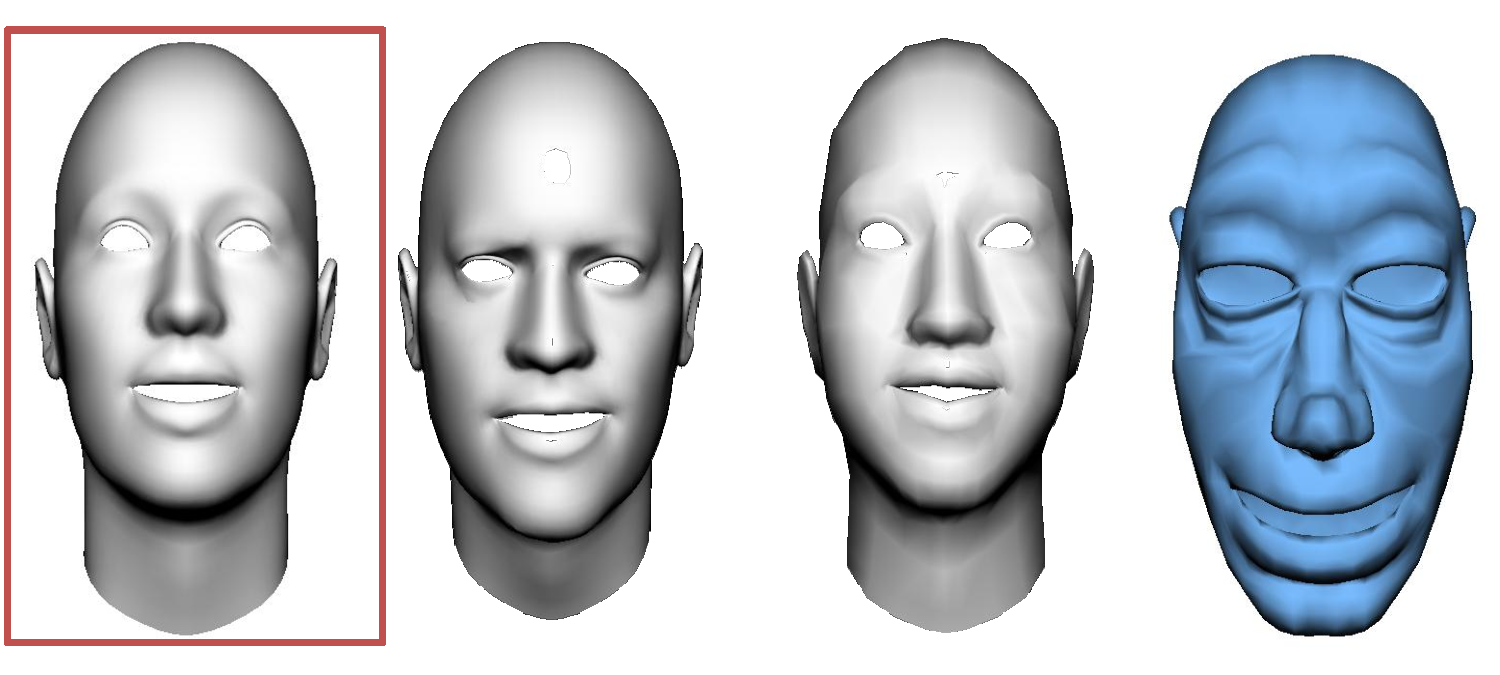
\includegraphics[width=0.5\linewidth]{figs/openSmile.pdf}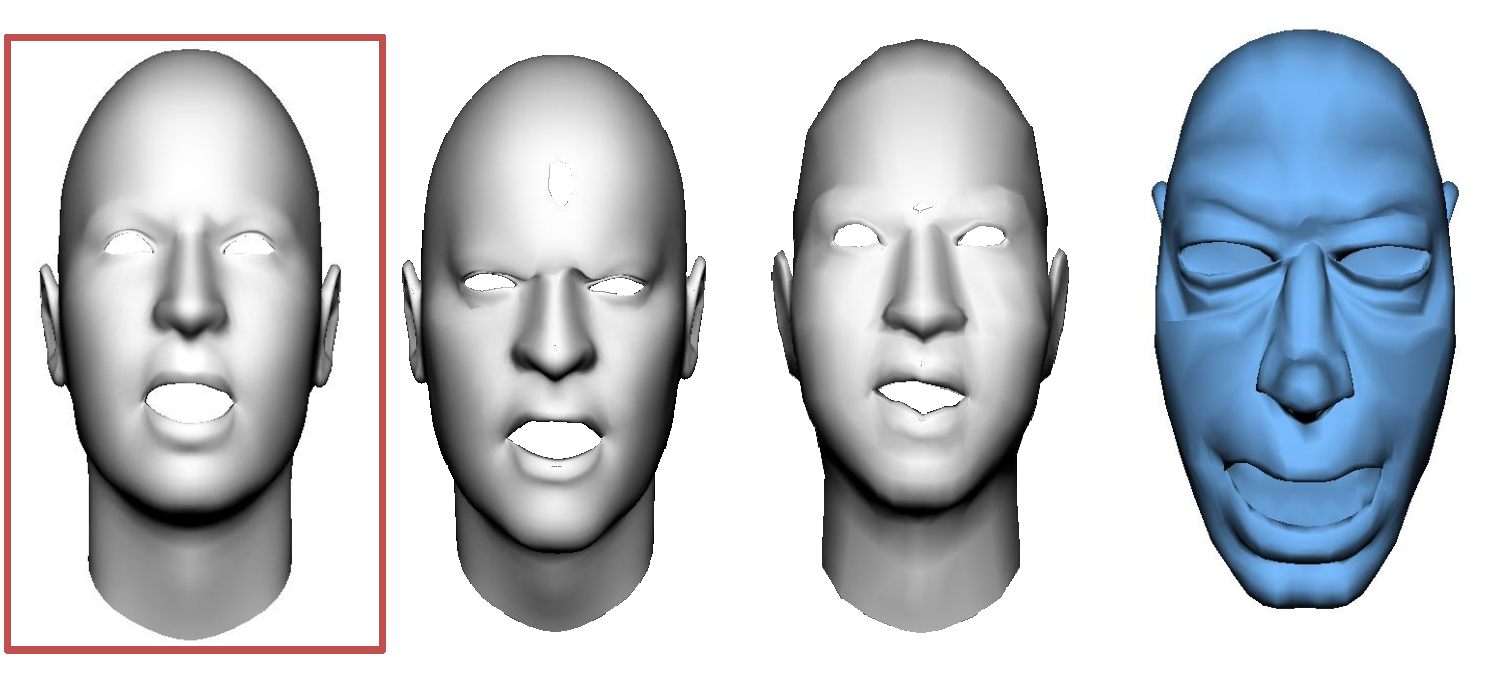
\includegraphics[width=0.5\linewidth]{figs/angryFace.pdf} 
  \caption{A figura de \emph{teaser} é opcional, e em geral usamos ela para mostrar alguns resultados visuais mais relevantes do trabalho (para "vender o peixe" visualmente).}
  \label{figura:teaser}
}


\abstract{O resumo de um artigo deve conter, em poucas palavras: uma frase que resume o objetivo principal, uma ou duas frases que explicam qual foi a metodologia e/ou principais técnicas utilizadas para alcançar este objetivo, como o resultado obtido foi avaliado e o resumo das principais conclusões/discussões obtidas pela avaliação dos resultados.

\smallskip
%pelo menos 3 palavras-chave relacionadas ao trabalho (pense como se fossem as hashtags para que seu trabalho seja encontrado)
\noindent \textbf{Palavras-chave:} Jogos Digitais; Animação Facial; \emph{Rigging} Facial; Transferência de Expressões.
} 